\section{Head Mapper}
%	* high order feature: arc heat change, influence of 2 order feature, feature template
%	* learning: MIRA, converge of training
%	* pseudocode of mapper(avoid circle) framework
%\KZ{Rephrase the following. What do you mean by attach? Also try not to be too casual, e.g., think about...}
%\BF{Mcdonald's example graph of decoding: ROOT John saw a dog yesterday which was a Yorkshire Terrier.}
In this section, we first give an example to explain how head mapper actually works. Then we explain
the features and scorer embeded in the head mapper. Finally, we describe the method to train the scorer model.

%\KZ{Figure needs to be restored to original one as some letters are missing.}

\begin{figure*}[th]
\centering
\epsfig{file=exampleparse_chg.eps, width=1.8\columnwidth}
\caption{Example Parse of head mapper}
%for the sentence ``\emph{John saw a dog yesterday which was a Yorkshire Terrier}". Red node is the child to be processed in every step; red arc is the final attachment from head to its dependent and dashed arc is left out to avoid circle in the parse tree.}
\label{fig:egparse}
\end{figure*}

\subsection{Parsing}
\figref{fig:egparse} shows the decoding process of the head mapper
for a non-projective example sentence previously used \cite{mcdonald2005non}.
%\KZ{You don't have to repeat the CoNNL format. It's not important.}
%Pseudocode shows how the head mapper works.
%Our decoder works just as the process in \figref{fig:egparse}.
%\BF{pseudocode of head mapper decoding and symbol explainations here}
A head mapper takes lexical information of a sentence and
a permutation sequence of words in that sentence as inputs.
The sequence of the sentence is:% from MaltParser:
$John_{1}\rightarrow a_{3}\rightarrow dog_{4}\rightarrow yesterday_{5}\rightarrow Yorkshire_{9}\rightarrow a_{8}\rightarrow was_{7}\rightarrow which_{6}\rightarrow Terrier_{10}\rightarrow saw_{2}$.
In step one, we look for the head of \textit{John} and
all the other words are potential candidate head. In order to measure
the probabilities of these candidate arcs, we introduce a scorer which
is the key idea of graph-based parsers. Judging from the scores
printed on every black arc in \figref{fig:egparse},
the red arc was eventually selected, i.e. $saw$ is taken to be the head
of $John$.  The process continues for the word \textit{a}, etc.

In practice, we maintain a disjoint set to ensure that
there are no cycles generated while parsing (e.g., in step 3 of
\figref{fig:egparse}),
so that the output is a dependency tree structure starting from
the ROOT node\footnote{A manually introduced node in dependency parsing task,
it is the root of a dependency tree}.
We also build a parse agenda to record the existing arcs which
provides the high order information for our scorer.
For a sentence with $N$ words, the final result consists of
($N+1$) nodes and constructed $N$ arcs.
%\KZ{You don't need to remind people over and over again this is a combination of
%MST and Malt. You just say what you did, if it's something that MST and Malt have
%done before, be very brief about this part, and give a citation. This paper
%is about your work, not about MST or Malt.}
%Both MaltParser and MSTParser treat projective and non-projective dependency tree discriminatively. MaltParser define an extra action SWAP to generate projectivization transformation of a non-projective dependency tree \cite{nivre2009non}.
%There is a drawback of MaltParser that it cannot generate non-projective output providing projective training set, because there are no SWAP action in oracle transitions. It is sensible to look into the relation between
%possible word pairs directly. But word order limits the word pairs considered in MaltParser. MSTParser employ Chu-Liu-Edmonds algorithm to decode non-projective cases \cite{mcdonald2005non}
%and Eisner algorithm to deal with projective trees\cite{mcdonald2005online}. Though Chu-Liu-Edmonds algorithm is a solution to unify projective and non-projective cases, it declines the accuracy while applying on projective trees. Our decoder also unifies these two situations and
%searches heads globally. It directly measures the relative closeness between every possible head and current processing word and generate non-projective tree naturally.
%Head mapper tries to map head for every word stepwise according to a given process sequence of words.
%\KZ{It makes sense to include an example here to illustrate the head-mapper.}

\subsection{Scorer and features}
%In order to simulate this process,
We introduce a linear arc scorer to measure the score of a directed arc.
The sum of all arc scores gives the final score of the whole parse tree.
%\BF{formula of arc score model}
%\[
%\text{Score}(\mathbf{y})=\displaystyle{\sum_{(i,j)\in\mathbf{y}}} \mathbf{w} \cdot \mathbf{f}(i,j)
%\]
%In this formula, $i,j$ are the indexes of an arc in parse tree $\mathbf{y}$. The inner product of arc feature vector $\mathbf{f}(i,j)$ and weight vector $\mathbf{w}$ represents score of an arc $(i,j)$. By summing up all the
%arc scores, we can get final score of the whole parse tree $\mathbf{y}$.
We currently use the same set of high-dimensional binary features as MSTParser,
%\BF{feature template table}
including second order features \cite{mcdonald2006online}.
%As the previous statement, feature scope in graph-based parser
%is limited by decoding algorithm and several works successfully
%adapt Eisner algorithm to include high order features .
Because of the deterministic decoding in our framework,
we can make use of existing arcs to guide later head mapping.
This kind of decoder gives us the flexibility of applying any
high order features explored by previous
works~\cite{carreras2007experiments,koo2010efficient,ma2012fourth}.

\subsection{Learning algorithm}
%\KZ{Again, you are making it sound like you only did some minor changes to MST.
%This is not the right style to write about your work. You can say we use a modified
%verion of MIRA~\cite{}, in which we did blah..}
%Based on different decoding and factoring methods, graph-based models employ different learning algorithms to induce the feature weights. Among them, variant perceptron algorithms are widely used \cite{kubler2009dependency}.
In this work, we adopt the iterative online training framework MIRA
(Margin Infused Relaxed Algorithm), which was used in the training process
of MSTParser~\cite{mcdonald2006online}. 
\cut{ 
The updating constraint is defined as
\begin{align*}
&\text{min}\|\mathbf{w}^{(i+1)}-\mathbf{w}^{(i)}\|\\
&\text{s.t. } s(\boldsymbol{x}_t,\boldsymbol{y}_t)-s(\boldsymbol{x}_t,\boldsymbol{y}')\ge L(\boldsymbol{y}_t,\boldsymbol{y}')
%\\&\forall \boldsymbol{y}'\in \text{dt}(\boldsymbol{x}_t)
\end{align*}
where $\mathbf{w}^{(i)}$ are the feature weights for the $i$-th iteration,
$\mathbf{x}_t$ and $\mathbf{y}_t$ are sentence and its gold parse tree,
respectively. $\mathbf{y}'$ is the output of our parser with $\mathbf{w}^{(i)}$ and
score margin is given out by a loss function $L$.
}
%On each update, MIRA attempts to keep the norm of the change to the parameter vector as small as possible, subject to
%correctly classifying the instance under consideration with a margin at least as large as the loss of the incorrect classifications \cite{mcdonald2005online}.
%\BF{this is the original sentence in this paper}
%Similarly, we define the loss function as the number of incorrect arcs to apply MIRA to dependency parsing and it
%is represented as following formula: \BF{Is this formula necessary ?}
%\BF{MIRA formula}
%\KZ{Don't like the following sentence.}
%From this definition, the only change we should make is replacing the exact inference decoder with our deterministic
%decoder.
Every time, we update the feature weights based on one sentence. The
decoder gives a greedy parse according to current feature weights.
By scoring the gold dependency tree and the current parse,
along with the number of incorrect arcs in the current parse,
MIRA updates to eventually converge to an optimal scorer.
The learning algorithm typically terminates after a few iterations.
%(\figref{fig:itertest}).
%\BF{Converge graph of head mapper}
%\begin{figure}[htp]
%\centering
%\epsfig{file=itertest.eps, width=\columnwidth}
%\caption{Accuracy curves on training set. \newline Test on first 100 sentence of WSJ senction 00.}
%\label{fig:itertest}
%\end{figure}
